\documentclass[dvipdfmx,10pt]{beamer}
%%%% Packages %%%%%
\usepackage{ipsj}
\usepackage{color}
\usepackage{amssymb}
\usepackage{amsmath}
\usepackage{amsthm}
\usepackage{multirow,bigdelim}
\newcommand{\la}{\leftarrow}
\newcommand{\Lra}{\Longrightarrow}
\newcommand{\Lla}{\Longleftarrow}
\newcommand{\Llra}{\Longleftrightarrow}
\newcommand{\lra}{\longrightarrow}
\newcommand{\dd}{\mathop{..}}
\newcommand{\range}[2]{\{#1\dd#2\}}
\newcommand{\imp}{\Rightarrow}
\newcommand{\equ}{\Leftrightarrow}
\renewcommand{\labelenumi}{(\arabic{enumi})}
\newcommand{\alldiff}{\textrm{alldifferent}}
\newcommand{\Alldiff}{\alldiff(x_1,x_2,\ldots,x_n)}
\newcommand{\SAT}{{\tt SAT}}
\newcommand{\UNSAT}{{\tt UNSAT}}
\newcommand{\Dom}{{\it Dom}}
% \newcommand{\p}[2]{p(#1,#2)}
\newcommand{\dE}[2]{p(#1=#2)}
\newcommand{\lE}[2]{p(#1^{(#2)})}
\newcommand{\oE}[2]{p(#1\le#2)}


\begin{document}
\title{解集合プログラミングを用いた\\クイーン支配問題の解法に関する考察}
\author{101830080 \quad 加藤 聖人}
\date{2021年度 卒業研究発表会 \\ 2022年2月18日}
\institute{番原研究室}

%
%表紙
%

\begin{frame}\frametitle{}
 \titlepage
\end{frame}

%
%支配集合問題について
%

\begin{frame}\frametitle{支配集合問題}
 \begin{block}{支配集合}
% 無向グラフ$G=(V,E)$の頂点の部分集合$S\subset V$に対して,
% 任意の頂点$u \in V\setminus S$にも辺$(u,v) \in E$が存在し,
% $v \in S$を満たすとき,$S$を$G$の\structure{支配集合}という.
無向グラフ$G=(V,E)$の頂点の部分集合$S\subset V$と,
その隣接頂点の集合との和集合が$V$と一致するとき,
$S$を$G$の\alert{\bf 支配集合}という.
\begin{itemize}
\item 支配集合の要素数を\structure{\bf サイズ}という.
\item サイズが最小の支配集合をグラフ$G$の\structure{\bf 最小支配集合}という.
\item 最小支配集合のサイズをグラフ$G$の\structure{\bf 支配数}といい,
  $\gamma(G)$で表す.
\end{itemize}
\end{block}

\begin{block}{支配集合問題}
  グラフ$G$と正の整数$k$が与えられたとき,サイズ$k$の支配集合が存在す
  るかどうかを判定する問題を\alert{\bf 支配集合問題}という.
  \begin{itemize}
  \item 支配集合問題は\structure{\bf NP完全}であることが知られている.
  \item 支配集合問題は,スケジューリング,電波塔配置問題などの問題に応
    用されている.
  \end{itemize}
 \end{block}
\end{frame}

%
%クイーン支配問題
%
\begin{frame}\frametitle{クイーン支配問題(Queen Domination Problem; QDP)}

  \begin{alertblock}{クイーン支配問題}\centering
    $n\times n$のクイーングラフ$Q_n$と正の整数$k$が与えられたとき,
    サイズ$k$の支配集合が存在するかどうかを判定する問題
 \end{alertblock}
 \vfill
 \begin{itemize}
 \item $Q_n$は$n\times n$のチェス盤について各マスを頂点とし,
   クイーンが移動できるマス同士が辺で結ばれているグラフである.
 \item $n\times n$の盤面に$k$個のクイーンを置いたとき,すべてのマスに
       1つ以上のクイーンが移動できるかどうかを判定する.
 \item 古くから研究されており,1862年に文献[Jaenisch,1862]で
   支配数$\gamma(Q_8)=5$が示されている.
 \item これまで,$1\leq n\leq 25$の支配数$\gamma(Q_n)$が求められ
   ている~\footnote{\url{https://oeis.org/A075458}}.
 \end{itemize}
\end{frame}
 
 
%
%クイーン支配問題の例
%

\begin{frame}{クイーン支配問題の例}
  \begin{exampleblock}{$Q_5$の最小支配集合}
  \begin{center}
   \scalebox{1.3}{
   \begin{tikzpicture}
 \draw[gray] (-1.25,-1.25)--(-1.25,1.25);
 \draw[gray] (-0.75,-1.25)--(-0.75,1.25);
 \draw[gray] (-0.25,-1.25)--(-0.25,1.25); 
 \draw[gray] (0.25,-1.25)--(0.25,1.25); 
 \draw[gray] (0.75,-1.25)--(0.75,1.25); 
 \draw[gray] (1.25,-1.25)--(1.25,1.25); 
 \draw[gray] (-1.25,-1.25)--(1.25,-1.25); 
 \draw[gray] (-1.25,-0.75)--(1.25,-0.75); 
 \draw[gray] (-1.25,-0.25)--(1.25,-0.25); 
 \draw[gray] (-1.25,0.25)--(1.25,0.25); 
 \draw[gray] (-1.25,0.75)--(1.25,0.75); 
 \draw[gray] (-1.25,1.25)--(1.25,1.25);
 \foreach \x in {-1,-0.5,0,0.5,1}
  \foreach \y in {-1,-0.5,0,0.5,1} 
  \fill (\x,\y) circle (0.03);
 \draw[magenta] (-1.25,1)--(1.25,1);
 \draw[magenta] (-1,1.25)--(-1,-1.25);
 \draw[magenta] (-1.25,1.25)--(1.25,-1.25);
 \draw[magenta] (-1.25,0.75)--(-0.75,1.25);
 \draw[blue] (-1.25,-1)--(1.25,-1);
 \draw[blue] (-0.5,-1.25)--(-0.5,1.25);
 \draw[blue] (-0.25,-1.25)--(-1.25,-0.25);
 \draw[blue] (-0.74,-1.25)--(1.25,0.74);
 \draw[yellow] (1,1.25)--(1,-1.25);
 \draw[yellow] (-1.25,0.5)--(1.25,0.5);
 \draw[yellow] (0.25,1.25)--(1.25,0.25);
 \draw[yellow] (-0.76,-1.25)--(1.25,0.76);
 \fill[magenta] (-1,1) circle (0.03);
 \fill[yellow] (1,0.5) circle (0.03);
 \fill[blue] (-0.5,-1) circle (0.03);
  \matrix[matrix of nodes,nodes={inner sep=0pt,text width=0.5cm,
align=center,minimum height=0.43cm}]{
 \textcolor{magenta}{\symqueen} & \quad & \quad & \quad & \quad \\
 \quad & \quad & \quad & \quad & \textcolor{yellow}{\symqueen} \\
 \quad & \quad & \quad & \quad & \quad \\
 \quad & \quad & \quad & \quad & \quad \\
 \quad & \textcolor{blue}{\symqueen} & \quad & \quad & \quad \\};
\end{tikzpicture}
 

   }
  \end{center}
 \end{exampleblock}
 \vfill
 \begin{itemize}
  \item 3個のクイーンを置いたとき,すべてのマスに1つ以上のクイーンが移動可能である.
  \item 2個以下の場合,すべてのマスにクイーンが移動することは不可能である.
  \item したがって,支配数は$\gamma(Q_{5})=3$となる.
 \end{itemize}
\end{frame}



%
%ASPについて
%

\begin{frame}\frametitle{解集合プログラミング(Answer Set Programming; ASP)}
  \begin{block}{}\centering
    ASP は論理プログラミングから派生した宣言的プログラミングパラダイム
    の一種である.
  \end{block}
  \vfill
  \begin{itemize}
  \item \structure{ASP言語}は一階論理に基づいた知識表現言語の一種である.
%  \item \structure{論理プログラム}は,ASP のルールの有限集合である.
  \item \structure{ASPシステム}は論理プログラムから
	安定モデル意味論[Gelfond and Lifschitz '88]に基づく
	解集合を計算するシステムである.
  \item 近年ではSAT技術を応用した高速ASPシステムが実現され,
	システム検証,プランニング,システム生物学など様々な
	分野への応用が拡大している.
 \end{itemize}
 \begin{alertblock}{支配集合問題に対してASPを用いる利点}
  \begin{itemize}
   \item ASP言語の高い表現力を活かし,支配集合問題の制約を簡潔に記述可能.
   \item 拡張性が高く,様々な定式化を簡単に試すことができる.
   \item 遷移問題への拡張も容易.
     % \item 個数制約を用いて,部分和を表す制約を簡潔に記述可能.
   % \item 高速な解列挙が可能.
  \end{itemize}
 \end{alertblock}
\end{frame}
 
%
%研究目的と研究内容
%

\begin{frame}\frametitle{研究目的}
 \begin{alertblock}{研究目的}\centering
  ASP技術を活用し,支配集合問題を効率よく解くソルバーの実現.
 \end{alertblock}

 \begin{itemize}
 \item 本研究ではクイーン支配問題を対象とする.
 \item SAT型制約ソルバーを用いた既存研究~[山本,2021]で提案された制約モ
   デルを応用する.
 \end{itemize}

 \begin{block}{研究内容}
  \begin{enumerate}
   \item クイーン支配問題を解く3種類のASP符号化を考案した.
     \begin{itemize}
     \item 基本符号化
     \item 改良符号化
     \item 部分和符号化
     \end{itemize}
   \item クイーン支配問題 ($Q_{n}: 1\leq n\leq 20$) を用いた評価実験を行った.
  \end{enumerate}
 \end{block}
\end{frame}

%
%符号化3つ
%

\begin{frame}{考案したASP符号化}

  \begin{block}{クイーン支配問題の制約}
    \begin{itemize}
    \item チェスの盤面上に$k$個のクイーンが配置される(個数制約)
    \item どのマスにも,1つ以上のクイーンが移動できる(移動制約)
    \end{itemize}
  \end{block}

  \begin{enumerate}
  \item \structure{\bf 基本符号化}
    \begin{itemize}
    \item マス$(i,j)$に対して,クイーンの有無を表すアトム$q(i,j)$を導
      入する.
    \item $q(i,j)$を用いて,個数制約を表現する.
    \item マスごとに移動制約を満たすかどうかチェックする.
    \end{itemize}
 \item \structure{\bf 改良符号化}
   \begin{itemize}
    \item 個数制約は基本符号化と同じ.
    \item 各行,各列,各対角線ごとにクイーンの有無を表す補助アトムを導入し,
      移動制約を満たすかどうかチェックする.      
   \end{itemize}
 \item \alert{\bf 部分和符号化}
   \begin{itemize}
   \item 各行,各列,各対角線ごとに
     クイーンの個数を表す補助アトムを導入し,
     個数制約と移動制約を表現する.
   \end{itemize}
 \end{enumerate}
\end{frame}


%
% 部分和符号化
%

\begin{frame}\frametitle{部分和符号化の特徴: 行方向の推論}
  \begin{itemize}
   % \item \structure{\bf アトム$q(i,j)$:} \quad $q(i,j)=\{0,1\}$
   % 	 \begin{itemize}
   % 	  \item アトム$q(i,j)$が1のとき,マス$(i,j)$にクイーン
   % 		が配置される.
   % 	 \end{itemize}
   \item \structure{\bf 補助アトム$r_i$:}\quad $r_{i}=\sum\limits_{j=1}^{n} 
	      q(i,j) \qquad (1 \leq i \leq n)$ 
	 \begin{itemize}
	  \item 行$i$上のクイーンの個数を$r_i$とする.
	 \end{itemize}
   \item \structure{\bf 個数制約:}\quad $\sum\limits_{i=1}^{n}r_{i} = k$
	 \begin{itemize}
	  \item 行ごとのクイーンの合計は盤面全体の数に一致する.
	 \end{itemize}
   \item \structure{\bf 移動制約:}\quad $(r_{i}>0 \vee c_{j}>0 \vee 
	 u_{i+j}>0 \vee d_{i-j} > 0) =1  \quad (1\leq i,j \leq n)$ 
	 \begin{itemize}
	  \item マス$(i,j)$にクイーンが1つ以上移動できる.
	  \item $c_{j}$, $u_{i+j}$, $d_{i-j}$は,
		列方向,対角線方向の補助アトム
	 \end{itemize}
  \end{itemize}
 \begin{exampleblock}{例:$Q_{5},k=3$}
  \begin{columns}
   \begin{column}{0.45\textwidth}
    \centering
    \scalebox{1}{
    \begin{tikzpicture}

 \tikzset{node/.style={circle,draw=black}}

 \definecolor{col_r}{RGB}{230,0,18}
 \definecolor{col_b}{RGB}{51,51,179}
 \definecolor{col_y}{RGB}{255,251,0}
 \definecolor{col_g}{RGB}{0,96,0}

 \node[node, fill=col_r!70] (node1){\textbf{1}};
 \node[node, fill=col_g!70, right=of node1] (node2){\textbf{2}};
 \node[node, fill=col_b!70, below=of node1] (node3){\textbf{3}};
 \node[node, fill=col_y!70, below=of node2] (node4){\textbf{4}};

 \foreach \u / \v in {node1/node2, node1/node3, node1/node4, node2/node3, node2/node4, node3/node4}
 \draw (\u) -- (\v);

\end{tikzpicture}
    }
   \end{column}
   \begin{column}{0.45\textwidth}
    \centering
    \scalebox{1}{
    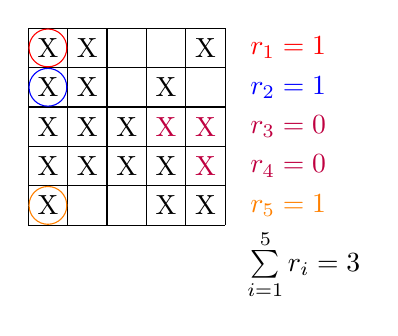
\begin{tikzpicture}
 \draw (0,0)--(2.5,0);
 \draw (0,0.5)--(2.5,0.5);
 \draw (0,1.0)--(2.5,1.0);
 \draw (0,1.5)--(2.5,1.5);
 \draw (0,2.0)--(2.5,2.0);
 \draw (0,2.5)--(2.5,2.5);
 \draw (0,0)--(0,2.5);
 \draw (0.5,0)--(0.5,2.5);
 \draw (1.0,0)--(1.0,2.5);
 \draw (1.5,0)--(1.5,2.5);
 \draw (2.0,0)--(2.0,2.5);
 \draw (2.5,0)--(2.5,2.5);
 \node (X) at (0.25,0.25) {X};
 \draw [orange] (0.25,0.25) circle[radius = 0.24];
 \node (X) at (0.25,0.75) {X};
 \node (X) at (0.25,1.25) {X};
 \node (X) at (0.25,1.75) {X};
 \draw [blue] (0.25,1.75) circle[radius = 0.24];
 \node (X) at (0.25,2.25) {X};
 \draw [red] (0.25,2.25) circle[radius = 0.24];
 \node (X) at (0.75,2.25) {X};
 \node (X) at (0.75,0.75) {X};
 \node (X) at (0.75,1.25) {X};
 \node (X) at (0.75,1.75) {X};
 \node (X) at (1.25,0.75) {X};
 \node (X) at (1.25,1.25) {X};
 \node (X) at (1.75,0.25) {X};
 \node (X) at (1.75,0.75) {X};
 \node (X) at (1.75,1.25) {\color{purple}X};
 \node (X) at (1.75,1.75) {X};
 \node (X) at (2.25,0.25) {X};
 \node (X) at (2.25,0.75) {\color{purple}X};
 \node (X) at (2.25,1.25) {\color{purple}X};
 \node (X) at (2.25,2.25) {X};
 \node (A) at (3.30,2.25) {\color{red}$r_{1} = 1$};
 \node (B) at (3.30,1.75) {\color{blue}$r_{2} = 1$};
 \node (M) at (3.30,1.25) {\color{purple}$r_{3} = 0$};
 \node (M) at (3.30,0.75) {\color{purple}$r_{4} = 0$};
 \node (C) at (3.30,0.25) {\color{orange}$r_{5} = 1$};
 \node (D) at (3.50,-0.50) {$\sum\limits_{i=1}^{5}r_{i}=3$};
\end{tikzpicture}
    }
   \end{column}
  \end{columns}
  \begin{itemize}
   \item 左の状態から,個数制約と移動制約により右の状態を推論できる.
  \end{itemize}
 \end{exampleblock}
\end{frame}


%
% 実験概要
%
\begin{frame}\frametitle{実験概要}
  \begin{block}{}\centering
    考案したASP符号化の有効性を評価するために実験を行った.    
  \end{block}
  \vfill
  \begin{itemize}
  \item \structure{\bf 比較するASP符号化}
    \begin{itemize}
    \item 基本符号化
    \item 改良符号化
    \item 部分和符号化
    \end{itemize}
  \item \structure{\bf クイーン支配問題}
    \begin{itemize}
    \item クイーングラフ $Q_{n}$ \quad ($1 \leq n \leq 20)$
    \item サイズ$k$には,充足可能(\textsf{SAT})なケースとし
      て既知の支配数$k=\gamma(Q_{n})$,
      充足不能(\textsf{UNSAT})なケースとして$k=\gamma(Q_{n})-1$ を使用.
    \end{itemize}
  \item \structure{\bf ASP システム:} \textit{clingo-5.5.0}
  \item \structure{\bf 制限CPU時間:} 3600秒 / 1問
  \item \structure{\bf 実験環境:} Mac mini, 3.2GHz 6コア Intel Core i7, 64GBメモリ
  \end{itemize}
\end{frame}


%
%実験結果(基本1,改良1,部分和2)
%

\begin{frame}\frametitle{実験結果: 求解に要した CPU 時間 (秒)}

 \begin{columns}
  \begin{column}{0.50\textwidth}
   \begin{table}[htbp]
     \caption{$k=\gamma(Q_{n})$ (\textsf{SAT})}
     \scalebox{0.7}{
     \centering 
 \begin{tabular}{c|c|r|r|r} \hline
  $n$ & $k$ & 基本 & 改良 & 部分和 \\ \hline
  10 & 4 & 14.400 & 21.232 & 3.005 \\
  11 & 4 & 54.674 & 123.488 & 32.540 \\
  12 & 5 & T.O. & 56.468 & 2.147 \\
  13 & 6 & T.O. & 1281.823 & 22.412 \\  
  14 & 7 & 2797.041 & 772.276 & 10.044 \\   
  15 & 8 & T.O. & T.O. & 275.683 \\  
  16 & 8 & T.O. & T.O. & \textbf{734.878} \\
  17 & 8 & T.O. & T.O. & T.O. \\
  18 & 8 & T.O. & T.O. & T.O. \\
  19 & 9 & T.O. & T.O. & T.O. \\
  20 & 10 & T.O. & T.O. & T.O. \\ \hline
 \end{tabular}}
   \end{table}
  \end{column}
  \begin{column}{0.50\textwidth}
   \begin{table}[htbp]
     \caption{$k=\gamma(Q_{n})-1$ (\textsf{UNSAT})}
    \scalebox{0.7}{
     \centering 
 \begin{tabular}{c|c|r|r|r} %\hline
  $n$ & $k$ & 基本 & 改良 & 部分和 \\ \hline
  10 & 4 & 10.280 & 8.929 & \alert{2.612} \\
  11 & 4 & 28.184 & 24.537 & \alert{3.427} \\
  12 & 5 & 2706.092 & 2673.241 & \alert{337.127} \\
  13 & 6 & T.O. & T.O. & T.O. \\  
  14 & 7 & T.O. & T.O. & T.O. \\   
  15 & 8 & T.O. & T.O. & T.O. \\  
  16 & 8 & T.O. & T.O. & T.O. \\
  17 & 8 & T.O. & T.O. & T.O. \\
  18 & 8 & T.O. & T.O. & T.O. \\
  19 & 9 & T.O. & T.O. & T.O. \\
  20 & 10 & T.O. & T.O. & T.O. \\ %\hline
 \end{tabular}}
   \end{table}
  \end{column}
 \end{columns} 
 \begin{itemize}
 \item 充足可能(\textsf{SAT})の問題では,部分和符号化が$n=16$まで解き,
   その優位性を確認できた.
 \item 充足不能(\textsf{UNSAT})の問題では,解けた問題数に差はなかったが,
   判定の要したCPU時間は部分和符号化が最も短かった.
 \end{itemize}
\end{frame}

%
%まとめと今後の課題
%

\begin{frame}\frametitle{まとめ}

  \begin{block}{}\centering
    ASP を用いたクイーン支配問題の解法について述べた.
  \end{block}
  \vfill
  \begin{enumerate}
  \item クイーン支配問題を解く3種類のASP符号化を考案した.
    \begin{itemize}
    \item ASPの表現力を活かして,クイーン支配問題を簡潔に記述できるこ
      とを確認した.
    \end{itemize}
  \item クイーン支配問題 ($Q_{n}: 1\leq n\leq 20$) を用いた評価実験を行った.
    \begin{itemize}
    \item 充足可能(\textsf{SAT})の問題について,
      部分和符号化が$n=16$まで解き,その優位性を確認できた.
    \end{itemize}
  \end{enumerate}
  \vfill
  \begin{block}{今後の課題}
    \begin{itemize}
    \item 支配集合問題を解くASP符号化の改良
      \begin{itemize}
      \item 現時点では,SAT型制約ソルバーを用いた既存研究~[山本,2021]
        と比較して性能面で劣っている.
      \end{itemize}
    \item 遷移問題への拡張
    \end{itemize}
  \end{block}
\end{frame}

%
%付録
%

%%%% 補助スライド
\appendix
\backupbegin

\begin{frame}{~}
 \centering
 - 補足用 -
\end{frame} 

%%%%%%%%%%%%%%%%%%%%%%%%%%%%%%%%%%%%%%%%%%%%%%%%%%
%% 電気制約
%%%%%%%%%%%%%%%%%%%%%%%%%%%%%%%%%%%%%%%%%%%%%%%%%%
\begin{frame}{補足 : 電気制約}
 \begin{itemize}
  \item \alert{電気制約}は,送電する電流$\cdot$電圧の適正範囲を保証する制約.
  \begin{itemize}
   \item 供給経路の各区間で許容電流を超えない.
   \item 電気抵抗による電圧降下が許容範囲を超えない.
   \item etc.
  \end{itemize}
  \item 電流と電圧が影響し合う\structure{実数ドメイン上の制約}によって表される.
		% \begin{itemize}
		%  		 \item 送電システム上の条件など.
		% \end{itemize}
  \item 実数ドメイン上の制約は,純粋なASPのみで扱うのは\alert{困難}.
		\begin{itemize}
		 \item 緩和問題として,変電所から供給できる家庭の数に上限をつける.
		 \item ASPMT技術により,ASPで得られた解について,
			   背景理論ソルバーと連携して実数ドメイン上の制約を調べる.
		\end{itemize}
 \end{itemize}
\end{frame}

%%%%%%%%%%%%%%%%%%%%%%%%%%%%%%%%%%%%%%%%%%%%%%%%%%
%% 基礎化
%%%%%%%%%%%%%%%%%%%%%%%%%%%%%%%%%%%%%%%%%%%%%%%%%%
\begin{frame}{補足 : ASPシステム}
 
 \vspace{-0.5cm}

 \begin{figure}[htbp]
  \centering
  %%%%%%%%%%%%%%%%%%%%%%%%%%%%%%%%%%%%%%%%%%%%%%%%%%
%% 基礎化の流れの図
%%%%%%%%%%%%%%%%%%%%%%%%%%%%%%%%%%%%%%%%%%%%%%%%%%
\begin{tikzpicture}

 \definecolor{edge}{RGB}{38,38,134}
 \definecolor{node}{RGB}{220,220,249}

 \definecolor{alert_edge}{RGB}{191,0,0}
 \definecolor{alert_node}{RGB}{249,200,200}

 \definecolor{ex_edge}{RGB}{0,96,0}
 \definecolor{ex_node}{RGB}{230,239,230}

 \def\nodespace{2.4cm}

 \tikzset{block/.style={rectangle, thick, draw=edge, fill=node, text width=3cm, 
 text centered, rounded corners, text width=2cm, minimum height=1.5cm}};

 \tikzset{alertblock/.style={rectangle, thick, draw=alert_edge, fill=alert_node, 
 text width=3cm, text centered, rounded corners, text width=1.5cm, minimum height=1.2cm}};

 \node[block](ikkai){一階ASP\\プログラム};

 \node[rectangle,rounded corners, thick, draw=ex_edge, fill=ex_node, 
 right=0.22*\nodespace of ikkai, minimum width=6cm, minimum height=3cm, 
 text centered, label=ASPシステム](sys){};

 \node[block, right=\nodespace of ikkai](meidai){命題ASP\\プログラム};
 \node[block, right=\nodespace of meidai](ASP){解集合};

 \node[right=0.6*\nodespace of ikkai, text width=1.5cm, 
 text centered, text=red, anchor=south](){基礎化\\ソルバー};
 \node[right=0.4*\nodespace of meidai, text width=1.5cm, 
 text centered, text=red, anchor=south](){解集合\\ソルバー};

 
 \foreach \u / \v / \n in {ikkai/meidai,meidai/ASP}
 \draw [thick,->] (\u) to (\v);

\end{tikzpicture}
 \end{figure}

 \vspace{-0.5cm}

 \begin{exampleblock}{}
  \begin{enumerate}
   \item 一階ASPプログラムを基礎化ソルバーによって,
		 命題ASPプログラムに\alert{基礎化}する.
   \item 命題ASPプログラムについて,SAT技術を応用した解集合ソルバーが解集合を探索する.
  \end{enumerate}
 \end{exampleblock}

\end{frame}
%%%%%%%%%%%%%%%%%%%%%%%%%%%%%%%%%%%%%%%%%%%%%%%%%%
%% ASPの構文
%%%%%%%%%%%%%%%%%%%%%%%%%%%%%%%%%%%%%%%%%%%%%%%%%%
\begin{frame}{ASPの構文}
  \begin{alertblock}{}\centering
    ASPの言語は論理プログラムをベースとしている~\footnotemark.
  \end{alertblock}
  \begin{itemize}
  \item \structure{\bf 論理プログラム}とは,以下の\structure{\bf ルール}の有限集合である.
    \begin{center}
      \begin{minipage}[c]{0.7\textwidth}
        \begin{block}{}\centering
          $a_0$\quad\code{:-}\quad$a_1$\code{,}\ldots\code{,}$a_m$\code{,}
          \ \code{not}~$a_{m+1}$\code{,}\ldots\code{,} \code{not}~$a_n$\code{.}
        \end{block}        
      \end{minipage}
   \end{center}\vfill
    $0 \leq m \leq n$ であり,各 $a_i$ はアトム,
    \code{not}は\structure{\bf デフォルトの否定},\\
    ``\code{,}''は連言(AND)を表す.``\code{:-}''の左辺を\structure{\bf ヘッド},
		右辺を\structure{\bf ボディ}と呼ぶ.
  \item \alert{\bf 直感的な意味}は,
    「$a_1,\ldots,a_m$がすべて成り立ち,
    $a_{m+1},\ldots,a_n$のそれぞれが成り立たないならば,
    $a_0$が成り立つ」である.
  \item ボディが空のルールを\structure{\bf ファクト}と呼び,``\code{:-}''は省略できる.
  \item ヘッドが空のルールを\structure{\bf 一貫性制約}と呼ぶ.例えば,\hspace{-1ex}
    ``\code{:-} $a_1$\code{,} \code{not}~$a_{2}$''は,
    「$a_1$が成り立つならば,$a_2$が成り立つ」を意味する.
  \end{itemize}
  \footnotetext{本発表では標準論理プログラムを単に論理プログラムと呼ぶ.}
\end{frame}
%%%%%%%%%%%%%%%%%%%%%%%%%%%%%%%%%%%%%%%%%%%%%%%%%%
%% ASPの拡張構文
%%%%%%%%%%%%%%%%%%%%%%%%%%%%%%%%%%%%%%%%%%%%%%%%%%
\begin{frame}{ASPの拡張構文}
\begin{alertblock}{}\centering
  組合せ問題を解くための便利な構文が用意されている.
\end{alertblock}
\begin{itemize}
 \item \structure{\bf 選択子}
   \begin{center}
     \code{\{}$a_1$\code{;}\ldots\code{;}$a_n$\code{\}}
   \end{center}
   アトム集合 $\{a_1,\dots,a_n\}$
   の任意の部分集合が成り立つことを意味する.
 \item \structure{\bf 個数制約}
   \begin{center}
     $lb$\ \code{\{}$a_1$\code{;}\ldots\code{;}$a_n$\code{\}}\ $ub$
   \end{center}
   $a_1,\dots,a_n$ のうち,
   $lb$個以上,$ub$個以下が成り立つことを意味する.
 \item \structure{\bf 重み付き個数制約}
   \begin{center}
     $lb$ \code{\#sum\{} $w_1$\code{:}$a_1$\code{;}\ldots\code{;}$w_n$\code{:}$a_n$ \code{\}} $ub$
   \end{center}
   $a_1,\dots,a_n$のうち,
   成り立つアトムの重み和が$lb$以上,$ub$以下になることを意味する.
\end{itemize}
\end{frame}
%%%%%%%%%%%%%%%%%%%%%%%%%%%%%%%%%%%%%%%%%%%%%%%%%%
%% 改良符号化 (到達可能性)
%%%%%%%%%%%%%%%%%%%%%%%%%%%%%%%%%%%%%%%%%%%%%%%%%%
\begin{frame}[fragile]{改良符号化: 到達可能性}
\begin{exampleblock}{}\small
\begin{lstlisting}
(1) { inForest(X,Y) } :- edge(X,Y).
\end{lstlisting}
\end{exampleblock}
\begin{itemize}
 \item (1) 各辺\code{(X,Y)について},根付き全域森に含まれること意味する \\
	  アトム\code{inForest(X,Y)}を導入する.
\end{itemize}
\begin{exampleblock}{}\small
\begin{lstlisting}
(2) reached(R,R) :- root(R).
(3) reached(X,R) :- reached(Y,R), inForest(Y,X).
(4) reached(X,R) :- reached(Y,R), inForest(X,Y).
\end{lstlisting}
\end{exampleblock}
\vfill
\begin{itemize}
\item アトム\code{reached(X,R)}は,ノード\code{X}が根ノード\code{R}から到達可能であることを意味する.
%\item (2) 各根ノード\code{R}について,自分自身から到達可能であることを表す.
\item (3) ノード\code{Y}が根ノード\code{R}から到達可能かつ,辺\code{(Y,X)}が根付き全域森に含まれるならば,
	  ノード\code{X}も同じ根ノード\code{R}から到達可能であることを表す.
\end{itemize}
\end{frame}
%%%%%%%%%%%%%%%%%%%%%%%%%%%%%%%%%%%%%%%%%%%%%%%%%%
%% 改良符号化 (根付き連結制約)
%%%%%%%%%%%%%%%%%%%%%%%%%%%%%%%%%%%%%%%%%%%%%%%%%%
\begin{frame}[fragile]{改良符号化: 根付き連結制約}
\begin{exampleblock}{}\small
\begin{lstlisting}
(5) :- node(X), not 1 { reached(X,R) } 1.
\end{lstlisting}
\end{exampleblock}
\vfill
\begin{itemize}
\item (5) 各ノード\code{X}について,ちょうど1つの根からのみ到達可能であることを意味する.
\end{itemize}
\end{frame}
%%%%%%%%%%%%%%%%%%%%%%%%%%%%%%%%%%%%%%%%%%%%%%%%%%
%% 改良符号化 (非閉路制約)
%%%%%%%%%%%%%%%%%%%%%%%%%%%%%%%%%%%%%%%%%%%%%%%%%%
\begin{frame}[fragile]{改良符号化: 非閉路制約}
\begin{minipage}[c]{1.01\textwidth}
\begin{exampleblock}{}\small
\begin{lstlisting}
(6) :- root(R),
       not 1 #sum{ 1,X:reached(X,R) ;
                  -1,X,Y:inForest(X,Y),reached(X,R),reached(Y,R)
                 } 1.
\end{lstlisting}
\end{exampleblock}
\end{minipage}
\vfill
\begin{itemize}
\item (6) 各連結成分の\structure{\bf ノード数と辺数の差が1}になることを意味する.
\item 各連結成分が\structure{\bf 木の性質}を満たすことにより,サイクルを持たない
	  ことを保証する.
\end{itemize}
\end{frame}
%%%%%%%%%%%%%%%%%%%%%%%%%%%%%%%%%%%%%%%%%%%%%%%%%%
%% ルール数の比較
%%%%%%%%%%%%%%%%%%%%%%%%%%%%%%%%%%%%%%%%%%%%%%%%%%
\begin{frame}{基礎化後のルール数}
  \begin{itemize}
  \item グラフのノード数を$|V|$,根ノードの数を$|R|$とする.
  \end{itemize}
  \begin{table}[t]
    \centering
    %%%%%%%%%%%%%%%%%%%%%%%%%%%%%%%%%%%%%%%%%%%%%%%%%%%%%%%%%%%%%%%%
\chapter{ハミルトン閉路問題および関連問題のASP符号化}\label{chap:proposal}
%%%%%%%%%%%%%%%%%%%%%%%%%%%%%%%%%%%%%%%%%%%%%%%%%%%%%%%%%%%%%%%% 

%%%%
\begin{figure}[h]
  \centering
  \thicklines
  \setlength{\unitlength}{1.2pt}
  \small\footnotesize\scriptsize
  \begin{picture}(280,57)(4,-10)
    \put(  0, 20){\dashbox(50,24){\shortstack{HCP問題\\インスタンス}}}
    \put( 60, 20){\framebox(50,24){変換器}}
    \put(120, 20){\dashbox(50,24){\shortstack{ASPファクト}}}
    \put(120,-10){\dashbox(50,24){\shortstack{ASP符号化\\(論理プログラム)}}}
    \put(180, 20){\framebox(50,24){ASPシステム}}
    \put(240, 20){\dashbox(50,24){\shortstack{HCP問題\\の解}}}
    \put( 50, 32){\vector(1,0){10}}
    \put(110, 32){\vector(1,0){10}}
    \put(170, 32){\vector(1,0){10}}
    \put(230, 32){\vector(1,0){10}}
    \put(170, +2){\line(1,0){4}}
    \put(174, +2){\line(0,1){30}}
  \end{picture}  
\caption{ASP を用いたハミルトン閉路問題(HCP)の解法}
\label{fig:arch}
\end{figure}
%%%%

%\begin{figure}[tbp]
\tikz{
  %1ノード目
  \path[draw=black, fill=blue!20, rounded corners=5pt]%線の設定
  node[at={(0.75,0.75)}] {問題}%文字を入れる
  (0,0) --(1.5,0) --(1.5,1.5) --(0,1.5) --cycle;%外周
  %2ノード目
  \path[draw=black, fill=blue!20, rounded corners=5pt, shift={(3,0)}]
  node[at={(0.75,0.75)}] {
    \begin{tabular}{c}
      ASP\\
      ファクト
    \end{tabular}
  }
  (0,0) --(1.5,0) --(1.5,1.5) --(0,1.5) --cycle;
  %3ノード目文字が複数行
  \path[draw=black, fill=green!20, rounded corners=5pt, shift={(6,0)}]
  node[at={(0.75,0.75)}] {
    \begin{tabular}{c}
      ASP\\
      システム
    \end{tabular}
  }
  (0,0) --(1.5,0) --(1.5,1.5) --(0,1.5) --cycle;
  %4ノード目文字が複数行
  \path[draw=black, fill=blue!20, rounded corners=5pt, shift={(9,0)}]
  node[at={(0.75,0.75)}] {解集合}
  (0,0) --(1.5,0) --(1.5,1.5) --(0,1.5) --cycle;
  %5ノード目文字が複数行
  \path[draw=black, fill=red!20, rounded corners=5pt, shift={(3,-3)}]
  node[at={(0.75,0.75)}] {
    \begin{tabular}{c}
      ASP\\
      符号化
    \end{tabular}
  }
  (0,0) --(1.5,0) --(1.5,1.5) --(0,1.5) --cycle;
  \draw[arrows=->] (1.5,0.75) --(3.0,0.75);
  \draw[arrows=->,shift={(3,0)}] (1.5,0.75) --(3.0,0.75);
  \draw[arrows=->,shift={(6,0)}] (1.5,0.75) --(3.0,0.75);
  \draw[arrows=->] (4.5,-2.25) --(6.0,0.5);
}
\caption{ASPを用いた解法}
\label{aspmethod}
\end{figure}


ASP を用いたハミルトン閉路問題および関連問題の解法について述べる.
図~\ref{fig:arch}に,解法の流れを示す.
与えられたハミルトン閉路問題は ASP ファクトに変換され,
ハミルトン閉路問題を解く ASP 符号化と結合され,
ASP システムによって解が計算される.
本論文では,ASP システムとして{\clingo}を用いる.

%%%%%%%%%%%%%%%%%%%%%%%%%%%%%%%%%%%%%%%%%%%%%%%%%%%%%%%%%%%%%%%%%%%%%%%
\section{ASPファクト形式}
%%%%%%%%%%%%%%%%%%%%%%%%%%%%%%%%%%%%%%%%%%%%%%%%%%%%%%%%%%%%%%%%%%%%%%%

%%%%%%%%%%%%%%%%%%%%%%%%%%%%%%
\begin{figure}[t]
\begin{center}
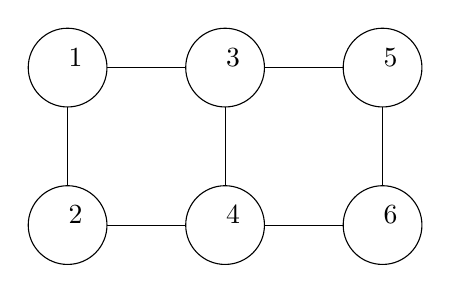
\begin{tikzpicture}
  %ノード1  
  \draw(4,2) circle (0.5)
  node[at={(4.1,2.1)}] {
    \begin{tabular}{c}
      1
    \end{tabular}
  };
  %ノード2  
  \draw(4,0) circle (0.5)
  node[at={(4.1,0.1)}] {
    \begin{tabular}{c}
      2
    \end{tabular}
  };
  %ノード3  
  \draw(6,2) circle (0.5)
  node[at={(6.1,2.1)}] {
    \begin{tabular}{c}
      3
    \end{tabular}
  };
  %ノード4  
  \draw(6,0) circle (0.5)
  node[at={(6.1,0.1)}] {
    \begin{tabular}{c}
      4
    \end{tabular}
  };
  %ノード5  
  \draw(8,2) circle (0.5)
  node[at={(8.1,2.1)}] {
    \begin{tabular}{c}
      5
    \end{tabular}
  };
  %ノード6  
  \draw(8,0) circle (0.5)
  node[at={(8.1,0.1)}] {
    \begin{tabular}{c}
      6
    \end{tabular}
  };
\draw(4,0.5) --(4,1.5);
\draw(6,0.5) --(6,1.5);
\draw(8,0.5) --(8,1.5);
\draw(4.5,0) --(5.5,0);
\draw(4.5,2) --(5.5,2);
\draw(6.5,0) --(7.5,0);
\draw(6.5,2) --(7.5,2);
\end{tikzpicture}

\caption{入力となる重み付き無向グラフの例}
\label{graphexample}
\end{center}
\end{figure}
%%%%%%%%%%%%%%%%%%%%%%%%%%%%%%

%%%%%%%%%%%%%%%%%%%%%%%%%%%%%%
\lstinputlisting[float=t,caption={%
図~\ref{graphexample}のASPファクト表現},%
captionpos=b,frame=single,label=code:graph_example.lp,%
numbers=none,%
breaklines=true,%
columns=fullflexible,keepspaces=true,%
basicstyle=\ttfamily\scriptsize]{code/graph_example.lp}
%%%%%%%%%%%%%%%%%%%%%%%%%%%%%%


本節では,最短ハミルトン閉路問題の例にとって,
入力となる重み付き無向グラフ(図~\ref{graphexample})の
ASP ファクト形式について説明する.
%
このグラフは,頂点数が6,辺の数が7であり,辺に付けられた値は距離を表す.
コード~\ref{code:graph_example.lp}に,ASPファクト形式を示す.
%
アトム\code{node/1}は頂点,\code{edge/2}は辺,\code{cost/3}は距離を表す.
例えば,\code{cost(1,2,3)}は,辺\code{edge(1,2)}の距離が3であることを
表している.

%%%%%%%%%%%%%%%%%%%%%%%%%%%%%%%%%%%%%%%%%%%%%%%%%%%%%%%%%%%%%%%%%%%%%%%
\section{ハミルトン閉路問題の ASP 符号化}\label{hamiltonianasp}
%%%%%%%%%%%%%%%%%%%%%%%%%%%%%%%%%%%%%%%%%%%%%%%%%%%%%%%%%%%%%%%%%%%%%%%

ハミルトン閉路問題は,与えられたグラフの全頂点をちょうど一度ずつ通る閉
路(ハミルトン閉路)が存在するかどうかを判定する問題である.
$G=(V,E)$にハミルトン閉路が存在する必要十分条件は,
以下の2つの制約を満たす部分グラフ$G'=(V,E')$が存在することである.

\begin{itemize}
\item $G'$の各頂点の次数が2 (次数制約)
\item $G'$が連結である (連結制約)
\end{itemize}

本論文では,前者を\textbf{次数制約},後者を\textbf{連結制約}と呼ぶ.
ハミルトン路問題は,ハミルトン閉路問題から始点と終点が一致するという閉
路の条件を取り除いたものである.
ハミルトン路問題では,次数制約は以下のように変わる.

\begin{itemize}
\item 始点と終点の次数が1,他の頂点の次数が2
\end{itemize}

以下では,ハミルトン閉路問題に対する3つの ASP 符号化
\textsf{undirected},\textsf{directed},\textsf{acyclicity}
を提案する.

%%%%%%%%%%%%%%%%%%%%%%%%%%%%%%%%%%%%%%%%%%%%%%%%%%%%%%%%%%%%%%%%%%%%%%%
\subsection{\textsf{undirected}符号化}
%%%%%%%%%%%%%%%%%%%%%%%%%%%%%%%%%%%%%%%%%%%%%%%%%%%%%%%%%%%%%%%%%%%%%%%

%%%%%%%%%%%%%%%%%%%%%%%%%%%%%%
\lstinputlisting[float=t,caption={%
\textsf{undirected}符号化},%
captionpos=b,frame=single,label=code:hamilton1.lp,%
numbers=left,%
breaklines=true,%
columns=fullflexible,keepspaces=true,%
basicstyle=\ttfamily\footnotesize]{code/hamilton1.lp}
%%%%%%%%%%%%%%%%%%%%%%%%%%%%%%

\textsf{undirected}符号化は,ハミルトン閉路問題の次数制約と連結制約を,
ASP の一貫性制約で表した基本的な符号化である.
コード~\ref{code:hamilton1.lp}に,\textsf{undirected}符号化を示す.
この符号化は,ハミルトン閉路問題とハミルトン路問題の両方に対応している.
符号化中の\code{s}は始点の頂点番号,\code{t}は終点の頂点番号を表し,こ
れらは実行時に与えられる.
ここでは,ハミルトン閉路問題(\code{s}=\code{t})の場合について説明する.

\begin{itemize}
\item 1行目のルールは,各辺\code{edge(X,Y)}に対して,その辺がハミルト
  ン閉路に含まれるかどうかを意味するアトム\code{in(X,Y)}を選択子を用い
  て導入している.
\item 次数制約は3行目のルールで表される.このルールは,
  各頂点\code{node(X)}に対して,その次数の和が2に等しいことを個数制約
  を使って表している.
\item 連結制約は11行目のルールで表される.
ある頂点\code{X}が始点\code{s}から到達可能であることを意味する補助アト
ム\code{reached(X)}を導入する.
8行目のルールは,始点\code{s}が到達可能あることを表している.
9行目のルールは,各辺\code{X}--\code{Y}に対して,その辺がハミルトン閉
路に含まれ(\code{in(X,Y)}),かつ,頂点\code{X}が始点から到
達可能であれば(\code{reached(X)}),\code{Y}も到達可能であることを表している.
10行目は9行目と同様であるが,辺\code{Y}--\code{X}の場合を表している.
11行目のルールは,各頂点\code{node(X)}が始点から到達可能でなければな
らないことを一貫性制約を使って表している.
\end{itemize}

%%%%%%%%%%%%%%%%%%%%%%%%%%%%%%%%%%%%%%%%%%%%%%%%%%%%%%%%%%%%%%%%%%%%%%%
\subsection{\textsf{directed}符号化}
%%%%%%%%%%%%%%%%%%%%%%%%%%%%%%%%%%%%%%%%%%%%%%%%%%%%%%%%%%%%%%%%%%%%%%%

%%%%%%%%%%%%%%%%%%%%%%%%%%%%%%
\lstinputlisting[float=t,caption={%
\textsf{directed}符号化},%
captionpos=b,frame=single,label=code:hamilton2.lp,%
numbers=left,%
breaklines=true,%
columns=fullflexible,keepspaces=true,%
basicstyle=\ttfamily\footnotesize]{code/hamilton2.lp}
%%%%%%%%%%%%%%%%%%%%%%%%%%%%%%

\textsf{directed}符号化は,\textsf{undirected}符号化をベースに,
与えられた無向グラフの各辺$u-v$に対して,2つの弧$u\rightarrow v$と
$v\rightarrow u$を対応させることで有向グラフ化して解く符号化である.
コード~\ref{code:hamilton2.lp}に,\textsf{directed}符号化を示す.
前節と同様に,ハミルトン閉路問題(\code{s}=\code{t})の場合について説明する.

\begin{itemize}
\item 1行目では,無向グラフの有向グラフ化を行う.
  与えられた無向グラフの各辺\code{edge(X,Y)}に対して,
  2つの弧\code{edge(X,Y)},\code{edge(Y,X)}を導入した.
\item 2行目のルールは,各弧\code{edge(X,Y)}に対して,その弧がハミルト
  ン閉路に含まれるかどうかを意味するアトム\code{in(X,Y)}を選択子を用い
  て導入している.
\item 次数制約は4,5行目のルールで表される.
  4行目では,各頂点\code{node(X)}に対して,
  その出次数が1に等しいことを個数制約を使って表している.
  5行目では,入次数について4行目と同様の制約を表す.
\item 連結制約は15行目のルールで表される.
  ある頂点\code{X}が始点\code{s}から到達可能であることを意味する
  補助アトム\code{reached(X)}を導入する.
  13行目のルールは,始点\code{s}が到達可能あることを表している.
  14行目のルールは,各弧\code{X}--\code{Y}に対して,その弧がハミルトン閉路
  に含まれ(\code{in(X,Y)}),かつ,頂点\code{X}が始点から
  到達可能であれば(\code{reached(X)}),\code{Y}も到達可能であることを表している.
  15行目のルールは,各頂点\code{node(X)}が始点から到達可能でなければ
  ならないことを一貫性制約を使って表している.
\item 18行目のルールは,解についての対称性を除去する.
  与えられた無向グラフ上の各ハミルトン閉路に対して,
  それを変換した有向グラフ上のハミルトン閉路は対称な2つが存在する.
  これによる解の重複を防ぐために,18行目のルールは,各弧\code{s}--\code{X},
  \code{Y}--\code{s}がハミルトン閉路に含まれるならば(\code{in(s,X),in(Y,s)}),
  \code{X < Y}でなければならないことを,一貫性制約を用いて表している
\end{itemize}

%%%%%%%%%%%%%%%%%%%%%%%%%%%%%%%%%%%%%%%%%%%%%%%%%%%%%%%%%%%%%%%%%%%%%%%
\subsection{\textsf{acyclicity}符号化}
%%%%%%%%%%%%%%%%%%%%%%%%%%%%%%%%%%%%%%%%%%%%%%%%%%%%%%%%%%%%%%%%%%%%%%%

%%%%%%%%%%%%%%%%%%%%%%%%%%%%%%
\lstinputlisting[float=t,caption={%
\textsf{acyclicity}符号化},%
captionpos=b,frame=single,label=code:hamilton3.lp,%
numbers=left,%
breaklines=true,%
columns=fullflexible,keepspaces=true,%
basicstyle=\ttfamily\footnotesize]{code/hamilton3.lp}
%%%%%%%%%%%%%%%%%%%%%%%%%%%%%%

\textsf{acyclicity}符号化は,\textsf{directed}符号化をベースに,
連結の制約に代わる部分閉路禁止制約を組込み非閉路制約で表現した符号化である.
コード~\ref{code:hamilton3.lp}に,\textsf{acyclicity}符号化を示す.
前節と同様に,ハミルトン閉路問題(\code{s}=\code{t})の場合について説明する.

\begin{itemize}
\item 1行目では,無向グラフの有向グラフ化を行う.
  与えられた無向グラフの各辺\code{edge(X,Y)}に対して,
  2つの弧\code{edge(X,Y)},\code{edge(Y,X)}を導入した.
\item 2行目のルールは,各弧\code{edge(X,Y)}に対して,その弧がハミルト
  ン閉路に含まれるかどうかを意味するアトム\code{in(X,Y)}を選択子を用い
  て導入している.
\item 次数制約は4,5行目のルールで表される.
  4行目では,各頂点\code{node(X)}に対して,
  その出次数が1に等しいことを個数制約を使って表している.
  5行目では,入次数について4行目と同様の制約を表す.
\item 部分閉路禁止制約は14行目のルールで表される.
  このルールは,始点でない各頂点\code{X},\code{Y}について,
  弧\code{X}--\code{Y}がハミルトン閉路に含まれるならば(\code{in(X,Y)}),
  そのような弧の集合をもつグラフが閉路をもたないことを,\code{#edge}宣言を用いて表す.
  ようするに,始点(終点)を含まないような閉路を禁止している.
\item 17行目のルールは,解についての対称性を除去する.
  与えられた無向グラフ上の各ハミルトン閉路に対して,
  それを変換した有向グラフ上のハミルトン閉路は対称な2つが存在する.
  これによる解の重複を防ぐために,17行目のルールは,各弧\code{s}--\code{X},
  \code{Y}--\code{s}がハミルトン閉路に含まれるならば(\code{in(s,X),in(Y,s)}),
  \code{X < Y}でなければならないことを,一貫性制約を用いて表している
\end{itemize}

%%%%%%%%%%%%%%%%%%%%%%%%%%%%%%%%%%%%%%%%%%%%%%%%%%%%%%%%%%%%%%%%%%%%%%% 
\section{最短ハミルトン閉路問題のASP符号化}\label{minexpl}
%%%%%%%%%%%%%%%%%%%%%%%%%%%%%%%%%%%%%%%%%%%%%%%%%%%%%%%%%%%%%%%%%%%%%%% 

%% %%%%%%%%%%%%%%%%%%%%%%%%%%%%%%
%% \lstinputlisting[caption =  最適化,label = minimize]{code/obj_minimize.lp}
%% %%%%%%%%%%%%%%%%%%%%%%%%%%%%%%

%%%%%%%%%%%%%%%%%%%%%%%%%%%%%%
\lstinputlisting[float=t,caption={%
最小化},%
captionpos=b,frame=single,label=code:obj_minimize.lp,%
numbers=left,%
breaklines=true,%
columns=fullflexible,keepspaces=true,%
basicstyle=\ttfamily\footnotesize]{code/obj_minimize.lp}
%%%%%%%%%%%%%%%%%%%%%%%%%%%%%%

最短ハミルトン閉路問題の目的関数は,
ハミルトン閉路を構成する各辺の距離の総和である.
コード\ref{code:obj_minimize.lp}は,
その目的関数の最小化を表す.
このコードは,各辺\code{edge(X,Y)}に対して,その辺がハミルトン閉路に
含まれ(\code{in(X,Y)}),その距離が\code{C}である時に(\code{cost(X,Y,C)}),
\code{C}の総和の最小化を,最小化関数を用いて表している.
.
%%%%%%%%%%%%%%%%%%%%%%%%%%%%%%
\lstinputlisting[float=t,caption={%
重み付き無向グラフの有向グラフ化},%
captionpos=b,frame=single,label=code:cost_both.lp,%
numbers=left,%
breaklines=true,%
columns=fullflexible,keepspaces=true,%
basicstyle=\ttfamily\footnotesize]{code/cost_both.lp}
%%%%%%%%%%%%%%%%%%%%%%%%%%%%%%

符号化directed,acyclicityについては,
与えられた無向グラフの各辺\code{edge(X,Y)}に対して,
2つの弧\code{edge(X,Y)},\code{edge(Y,X)}を導入した.
各辺の距離もこれに対応させるために,コード\ref{code:cost_both.lp}
を追加した.
このルールは,各辺\code{X}--\code{Y}の距離を表す\code{cost(X,Y,C)}について,
\code{cost(Y,X,C)}を導入する.
これにより,与えられた無向グラフの各辺\code{edge(X,Y)}の重み\code{C}が
2つの弧\code{edge(X,Y)},\code{edge(Y,X)}にも付与された.

%%%%%%%%%%%%%%%%%%%%%%%%%%%%%%%%%%%%%%%%%%%%%%%%%%%%%%%%%%%%%%%%%%%%%%% 
\section{コスト制約付きハミルトン閉路のASP符号化}
%%%%%%%%%%%%%%%%%%%%%%%%%%%%%%%%%%%%%%%%%%%%%%%%%%%%%%%%%%%%%%%%%%%%%%% 

%%%%%%%%%%%%%%%%%%%%%%%%%%%%%%
\lstinputlisting[float=t,caption={%
コスト制約},%
captionpos=b,frame=single,label=code:cost_constraint.lp,%
numbers=left,%
breaklines=true,%
columns=fullflexible,keepspaces=true,%
basicstyle=\ttfamily\footnotesize]{code/cost_constraint.lp}
%%%%%%%%%%%%%%%%%%%%%%%%%%%%%%

コスト制約付きハミルトン閉路問題は
ハミルトン閉路問題に,距離の総和が所与の閾値以下 (または以上) であること
を制約条件として付加した問題である.
コード\ref{code:const_constraing.lp}のルールは,その制約を表す.
ルール中の\code{c}は閾値を表し,これは実行時に与えられる.
このルールは,各辺\code{edge(X,Y)}に対して,その辺がハミルトン閉路に
含まれ(\code{in(X,Y)}),その距離が\code{C}である時に(\code{cost(X,Y,C)}),
\code{C}の総和が\code{c}以下でなければならないことを,
一貫性制約と重み付き個数制約を用いて表す.

また,\ref{minexpl}と同様に,
符号化directed,acyclicityについては,
アトム\code{cost}についても有向グラフ化に
対応させるためにコード\ref{code:cost_both.lp}を追加した.
%%%%%%%%%%%%%%%%%%%%%%%%%%%%%%%%%%%%%%%%%%%%%%%%%%%%%%%%%%%%%%%%%%%%%%%

%%% Local Variables:
%%% mode: latex
%%% TeX-master: "paper"
%%% End:

  \end{table}
\end{frame}

%%%%%%%%%%%%%%%%%%%%%%%%%%%%%%%%%%%%%%%%%%%%%%%%%%
%% ASPのコード
%%%%%%%%%%%%%%%%%%%%%%%%%%%%%%%%%%%%%%%%%%%%%%%%%%
\begin{frame}[fragile]{補足 : 根付き全域森 基本符号化}
%%%%%%%%%%%%%%%%%%%%%%%%%%%%%%%%% 
\lstinputlisting[frame=single,label=code:roop,%
xleftmargin=1zw,%
xrightmargin=1zw,%
numbersep=5pt,%
numbers=left,%
breaklines=true,%
columns=fullflexible,keepspaces=true,%
basicstyle=\ttfamily\scriptsize]{code/srf1.lp}
%%%%%%%%%%%%%%%%%%%%%%%%%%%%%%%%%
\end{frame}

\begin{frame}[fragile]{補足 : 遷移問題 シングルショット符号化}

\begin{multicols*}{2}
%%%%%%%%%%%%%%%%%%%%%%%%%%%%%%%%% 
\lstinputlisting[frame=single,label=code:roop,%
xleftmargin=1zw,%
xrightmargin=1zw,%
numbersep=5pt,%
numbers=left,%
breaklines=true,%
columns=fullflexible,keepspaces=true,%
basicstyle=\ttfamily\tiny]{code/trans-const.lp}
%%%%%%%%%%%%%%%%%%%%%%%%%%%%%%%%%
\end{multicols*}
\end{frame}

\begin{frame}[fragile]{補足 : 遷移問題 マルチショット符号化}
\begin{multicols*}{2}
%%%%%%%%%%%%%%%%%%%%%%%%%%%%%%%%%
\lstinputlisting[frame=single,label=code:incmode,% 
xleftmargin=1zw,%
xrightmargin=1zw,%
numbersep=5pt,%
numbers=left,%
breaklines=true,%
columns=fullflexible,keepspaces=true,%
basicstyle=\ttfamily\tiny]{code/dnet-trans.lp}
%%%%%%%%%%%%%%%%%%%%%%%%%%%%%%%%% 
\end{multicols*}
\end{frame}

\backupend


\end{document}
%%% Local Variables:
%%% mode: japanese-latex
%%% TeX-master: t
%%% End:
